\section{Authentication and Identity}

\begin{frame}
\frametitle{Authentication vs Identity}
\begin{block}{Identity}
The identity of somebody/something is who/what he/it is.
\end{block}
\begin{block}{Authentication} Authentication is the process of
  verification that an individual or an entity is who it claims to
  be \textit{(OWASP)}. 
\end{block}
\end{frame}

%------------------------------------------------

\begin{frame}
\frametitle{Why authentication?}

Authentication is needed when you want to transmit confidential
information, you want to be sure that your correspondant isn't
impersonated by somebody else.

Authentication by itself doesn't mean confidentiality as it doesn't
prevent eavesdropping.

\end{frame}


%------------------------------------------------
\subsection{Different means of authentication}

%------------------------------------------------
\begin{frame}
\frametitle{Passwords}

\begin{itemize}
\item The most common form of authentication
\item Password should be easily changeable
\item Peoples should have different passwords for different services
\item Complexity must be sufficient
\end{itemize}
\end{frame}


%------------------------------------------------

\begin{frame}
\frametitle{Password complexity}

Enforcing a minimum password strength:
\begin{itemize}
\item State the rules clearly(e.g. minimum 10 character, minimum a
  capital letter, \ldots)
\item Check the complexity in the browser to prevent him to submit a
  form with an ``invalid'' password
\item Check again on the server side
\item If the password doesn't comply, give all the violated rules in
  the error message.
\end{itemize}

\begin{figure}
  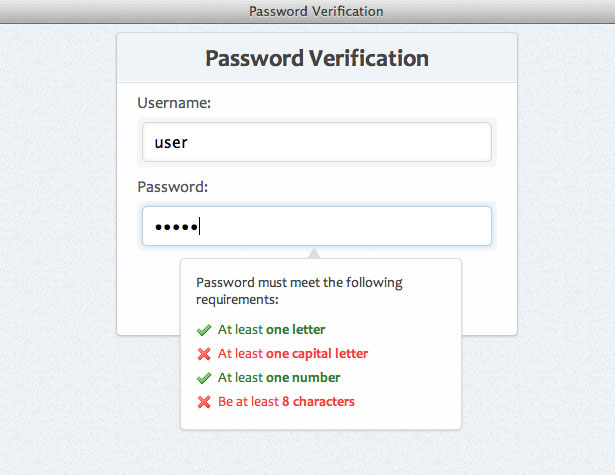
\includegraphics[width= 0.3\linewidth]{img/browserPasswordValidation.jpg}
\end{figure}

\end{frame}

%------------------------------------------------


\begin{frame}
\frametitle{One time passwords}

One time password (OTP for short) are passwords which are valid only
once. 
\begin{itemize}
\item Prevent replay attack.
\item Main difficulty: giving the user his passwords. 
\item Often cause logistical problems 
\item Used mainly by those who can afford big infrastructure (States,
  banks, other big companies, \ldots)
\end{itemize}
\end{frame}

%------------------------------------------------

\begin{frame}
\frametitle{One time passwords: choosing and distribution}

To avoid prediction, passwords must be chosen using a randow or at
least pseudorandom way.

There are various ways to distribute OTPs:
\begin{itemize}
\item If OTP generation is time based. Password are only valid for a
  short time. The generation can be done by a small electronic
  device which can be carried by the user.
\begin{figure}
  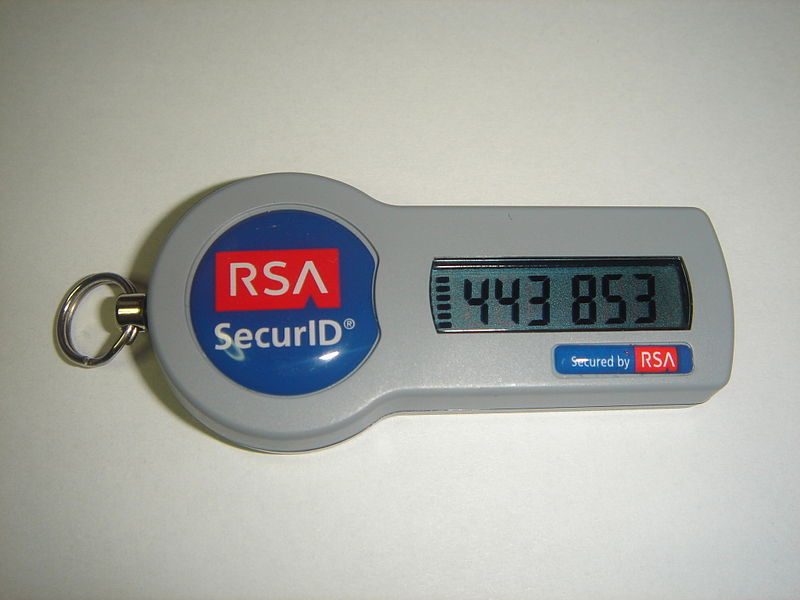
\includegraphics[width= 0.3\linewidth]{img/SecureID_token_new.JPG}
\end{figure}
\item You can send them out-of-band to the user (by SMS, mail, \ldots)
\item You can use a software on mobile phone that generate the passwords
\end{itemize}
\end{frame}

%------------------------------------------------

\begin{frame}
\frametitle{Certificates}
A trusted authority (Certification Authority) issues certificates to
confirm the ID of something. Those certificates may be of varying
quality and are most often used in SSL/TLS by web browsers.
\begin{figure}
  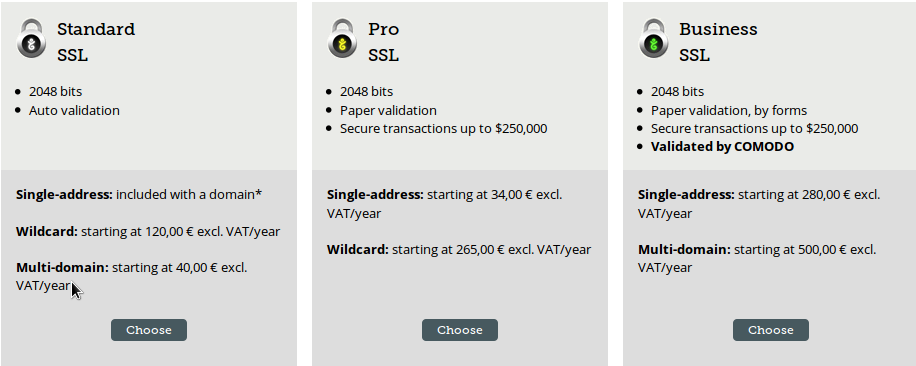
\includegraphics[width= 0.8\linewidth]{img/certificatesVariety.png}
\end{figure}
\end{frame}

%------------------------------------------------

\begin{frame}[fragile]
\frametitle{Certificates: What are they made of?}
Classical web certificates are using X.509 v3 standard.

\small
\begin{verbatim}

Certificate:
   Data:
       Version: 1 (0x0)
       Serial Number: 7829 (0x1e95)
       Signature Algorithm: md5WithRSAEncryption
       Issuer: C=ZA, ST=Western Cape,...
               OU=Certification Services Division,
               CN=Thawte Server CA/emailAddress=...
       Validity   
           Not Before: Jul  9 16:04:02 1998 GMT
           Not After : Jul  9 16:04:02 1999 GMT
\end{verbatim}

\end{frame}

%------------------------------------------------


\begin{frame}[fragile]

\small
\begin{verbatim}
       Subject: C=US, ST=Maryland,...
                OU=FreeSoft, CN=www.freesoft.org/emailAddress=...
       Subject Public Key Info:
           Public Key Algorithm: rsaEncryption
           RSA Public Key: (1024 bit)
               Modulus (1024 bit):
                   00:be ...:41:8f
               Exponent: 65537 (0x10001)
   Signature Algorithm: md5WithRSAEncryption
       93:5f...:68:9f
\end{verbatim}

\end{frame}

%------------------------------------------------


\begin{frame}
\frametitle{Certificates: How are they used?}
Certificates are often used as a mean to distribute key in a public
key infrastructure. A typical exemple is for SSL/TLS in web browsers.
\begin{figure}
  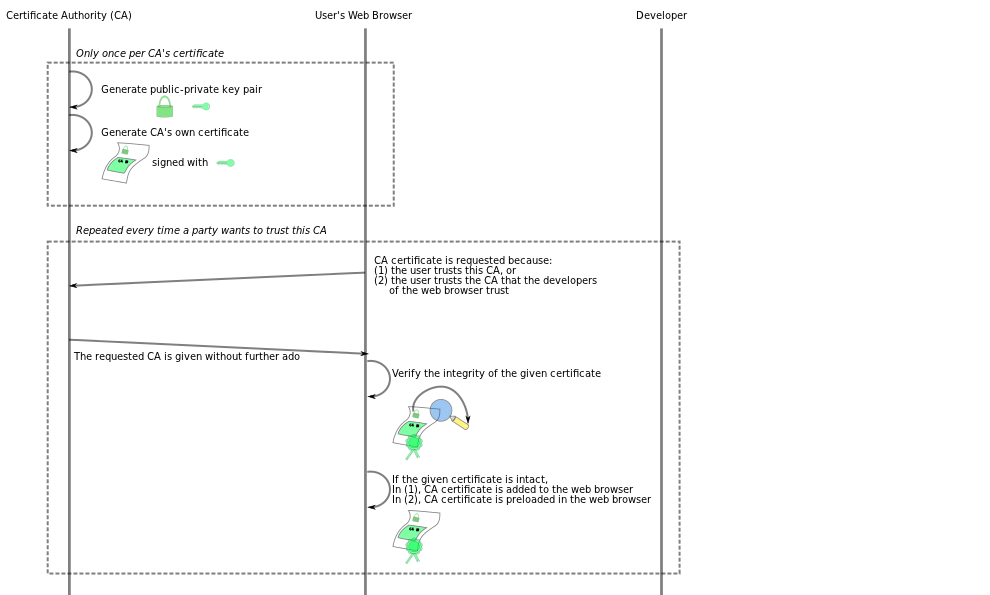
\includegraphics[width= 0.9\linewidth]{img/Usage-of-Digital-CertificatePart1.png}
\end{figure}

\end{frame}

%------------------------------------------------

\begin{frame}

\begin{figure}
  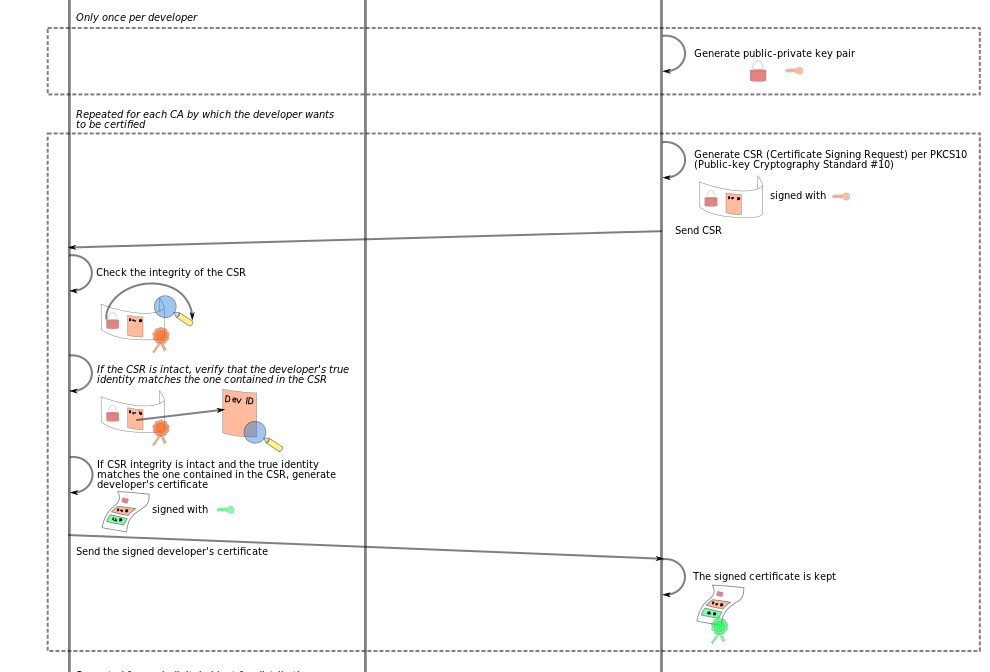
\includegraphics[width= 0.9\linewidth]{img/Usage-of-Digital-CertificatePart2.png}
\end{figure}

\end{frame}

%------------------------------------------------

\begin{frame}

\begin{figure}
  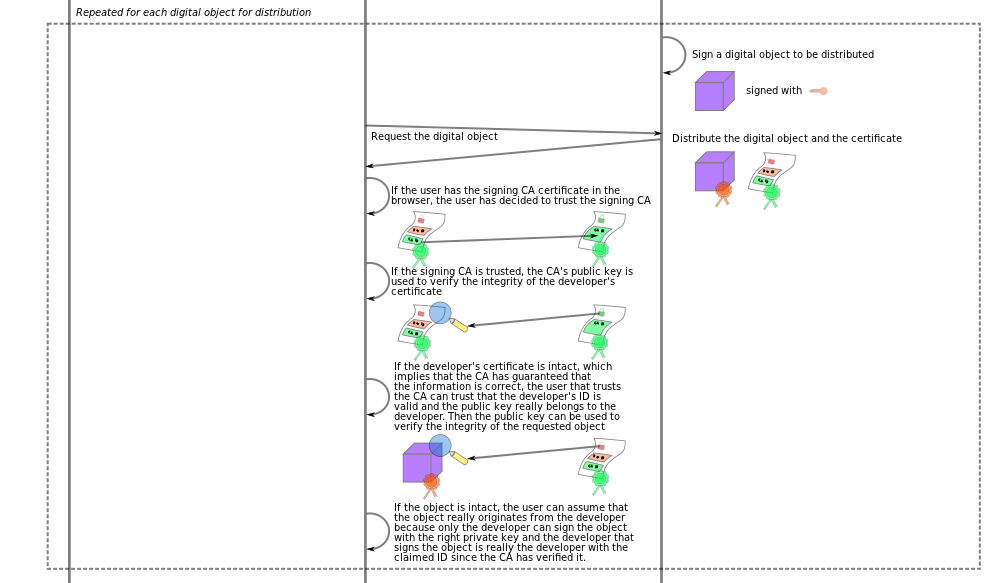
\includegraphics[width= 0.9\linewidth]{img/Usage-of-Digital-CertificatePart3.png}
\end{figure}
\textit{Wikipedia}
\end{frame}

%------------------------------------------------

\begin{frame}
\frametitle{Certificates: Two way authentication}

\begin{itemize}
\item In the previous scenario we have shown that the browser autenticates
the server but the opposite isn't true.

\item It's possible for both participant to authenticate \ldots

\item \ldots but it's more complicated: two good one way
  authentication don't make a valid two way authentication
\end{itemize}

\end{frame} 

%------------------------------------------------

\begin{frame}
\frametitle{Tokens}

\begin{block}{Token} Token are something which ownership gives a form
  of authentication.
\end{block}
\begin{itemize}
\item In our everyday life, token can take various forms: keys, bank card,
badges, \ldots
\item In electronic authentication schemes they are most often smart
  card or digipass
\end{itemize}
\end{frame}

%------------------------------------------------

\begin{frame}
\frametitle{Multi factor authentication}
 An application should use at least two factors of
 authentication. Those factors can be:
\begin{itemize}
\item what the authenticated entity is (biometrics, \ldots),
\item what it owns (a bank card, \ldots) 
\item or what he knows (a password, a pin code, \ldots)
\end{itemize}
\end{frame}

%------------------------------------------------

\subsection{Signature challenge}

%------------------------------------------------
\begin{frame}
\frametitle{Signature challenge: principle}

\begin{itemize}
\item An authentication based upon ``answering'' a question about a secret
known by the participants. For example, when I encrypt something (a nonce)
with my correspondent's public key and ask him for the decrypted and encrypted
message.

\item This form of authentication is often used to sign online
  transaction.
\end{itemize}

\end{frame}
%------------------------------------------------

\subsection{Single sign-on}

%------------------------------------------------
\begin{frame}
\frametitle{Single sign-on: principle}

\begin{block}{Single sign-on}
Single sign-on (SSO) is a property of access control of multiple
related, but independent software systems. With this property a user
logs in once and gains access to all systems without being prompted to
log in again at each of them. \textit{Wikipedia}
\end{block}

\end{frame}
%------------------------------------------------

\begin{frame}
\frametitle{Single sign-on: pro and cons}

\begin{block}{Pro}
\begin{itemize}
\item Easier for the user
\item Not trivial to build a secure authentication scheme
\item If they have only one password users tend to treat it with more care
\item Enter the password less often
\end{itemize}
\end{block}

\begin{block}{Cons}
\begin{itemize}
\item All your eggs in the same basket (impact if compromised)
\item You are dependant upon your provider (confidence, availability, \ldots)
\end{itemize}
\end{block}

\end{frame}

%------------------------------------------------

\subsection{Kerberos}

%------------------------------------------------

\begin{frame}
\frametitle{Kerberos}

Kerberos is a SSO developped at MIT to solve the problem of allowing
some users to use restricted ressources. MIT provide a free
implementation of the protocol but it's also found in many commercial
products.

\end{frame}

%------------------------------------------------

\begin{frame}
\frametitle{Kerberos: How it works}

\begin{figure}
  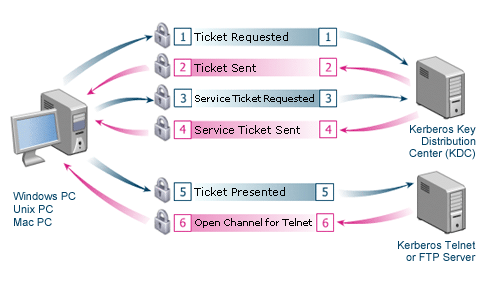
\includegraphics[scale = 0.35]{img/kerberos.png}
\end{figure}
\textit{Wikipedia}
\end{frame}

%------------------------------------------------
\subsection{Provider extensions}
%------------------------------------------------

\begin{frame}
\frametitle{Provider extensions}
\begin{itemize}
\item Single sign-on is provided for free by organisation like Facebook, OpenID and
Google to other websites for free.
\item The usage of those services is usually much easier for the
  developper than developping his own sign-on mechanism.
\item But it ties you to this provider so some sites use services from
  different organisations
\end{itemize}

\end{frame}

%------------------------------------------------
\subsection{Compromised authentication mean}
%------------------------------------------------

\begin{frame}
\frametitle{Compromised authentication mean}
 When you implement authentication you have to take into account that
 the user may loose its authentication mean or it can get stolen. So,
 you should be able to:

\begin{itemize}
\item Deactivate a compromised authentication mean,
\item Authenticate the user by an uncompromised mean,
\item Give him a new primary authentication mean.
\end{itemize}

\end{frame}

%------------------------------------------------

\begin{frame}
\frametitle{Example: Lost password}
 If one of your users loose his password, he has to get a new one but
 doing this in a secure way can be challenging. Here is a procedure
 that you can follow.

\begin{itemize}
\item use some predefined security questions,
\item send a token over a side channel,
\item allow the user to change password,
\item confirm change
\end{itemize}

\end{frame}
%------------------------------------------------
